\section{The heat equation with an explicit Euler}
  \label{section:applications:heat-equation}

\chapterDescription
  {
    60 minutes.
  }
  {
    Chapter \ref{chapter:quickstart}.
  }

In this section, we sketch how to realise a heat equation solver for
\[
  \partial _t u - \nabla (\epsilon \nabla) u = 0
\]
that is based
upon an explicit Euler.
It uses the spacetree as computational grid.


\subsection{Preparation}

We create an empty project with the PDT (\texttt{--create-project myproject
myproject}) and first adopt our cell and vertex data structure such that each
cell holds an $\epsilon$ value and each vertex holds the current and previous
solution.

\begin{code}
Packed-Type: short int;
class myproject::dastgen::Vertex {
  parallelise persistent double  u;
  discard                double  oldU;
};
\end{code}


\begin{code}
Packed-Type: short int;
class myproject::dastgen::Cell {
  persistent double epsilon;
};
\end{code}


\noindent
Furthermore, we make the code's state hold the solver's time step size. We will
write the code such that it works in 2d and 3d. All the pictures are done for a
3d setup. To run with other dimensions, you have to adopt your makefile
accordingly.


\begin{code}
Packed-Type: short int;
class myproject::dastgen::State { 
  persistent parallelise double dt;
};
\end{code}


\noindent
We do not use any sophisticated plotting routines and thus rely in some plotters
that are available out-of-the-box for Peano.
We also require only two mappings: one for the setup, one for the time stepping. 
Depending on our personal choices, we combine them with plotting features or
not\footnote{There is a known issue with the coding standards in Peano/PDT
which can be avoided a priori if all read and write attributes start with an
uppercase---even though they might be defined with lowercase in the def file.}.

\begin{code}
omponent: ExplicitEulerForHeatEquation
namespace: ::myproject
vertex:
  dastgen-file: Vertex.def
  read scalar(double): U
  read scalar(double): OldU
  write scalar(double): U
cell:
  dastgen-file: Cell.def
state:
  dastgen-file: State.def
event-mapping:
  name: CreateGrid
event-mapping:
  name: TimeStep
adapter:
  name: CreateGrid
  merge-with-user-defined-mapping: CreateGrid
adapter:
  name: TimeStep
  merge-with-user-defined-mapping: TimeStep
adapter:
  name: CreateGridAndPlot
  merge-with-user-defined-mapping: CreateGrid
  merge-with-predefined-mapping: VTKPlotCellValue(epsilon,getEpsilon,eps)
  merge-with-predefined-mapping: VTKPlotVertexValue(initialSetup,getU,u)
adapter:
  name: TimeStepAndPlot
  merge-with-user-defined-mapping: TimeStep
  merge-with-predefined-mapping: VTKPlotVertexValue(result,getU,u)
\end{code}

\noindent
To translate this file, you need the corresponding predefined mappings that are 
held in the repository or on the webpage.
To find out what the arguments of the predefined mappings mean, please have a 
look into the corresponding template header files.
We note that we write out epsilon only throughout the setup phase. 
It does not make sense to plot each each iteration, as this material parameter
does not change in time.
We furthermore note that we add some \texttt{read} and \texttt{write}
statements.
They make the PDT generate helper methods that allow us within each cell to
access all $u$ values of a cell as one vector.



\subsection{Making the plotter work}

This code so far does not compile. It complains with

\begin{code}
> make -f myproject/makefile
--- This is Peano 3 ---
g++ -DDim3 [...] -c myproject/adapters/CreateGridAndPlot2VTKPlotCellValue_0.cpp -o \
myproject/adapters/CreateGridAndPlot2VTKPlotCellValue_0.o 
[...]  In member function ‘void [...]::CreateGridAndPlot2VTKPlotCellValue_0::enterCell([...])’:
[...] error: ‘class myproject::Cell’ has no member named ‘getEpsilon’
     _cellValueWriter->plotCell(cellIndex,fineGridCell.getEpsilon() );
                                                       ^
make: *** [myproject/adapters/CreateGridAndPlot2VTKPlotCellValue_0.o] Error 1
\end{code}

\noindent
This is correct. 
We have told the predefined mapping that there would be an opteration
\texttt{getEpsilon} to print cell data, but we have not provided one yet.
A similar reasoning holds for the plotting of the actual solution.
Therefore, we add 

\begin{code}
void myproject::Cell::init() {
  _cellData.setEpsilon( 1.0 + static_cast<double>(rand() % 100)/100.0 );
}

double myproject::Cell::getEpsilon() const {
  return _cellData.getEpsilon();
}
\end{code}

\noindent
This snippet also allows us to initialise a cell with a random value from
$(1,2)$.


\begin{remark}
An initialisation of the cell's $\epsilon$ in the default constructor does not
work because of the flyweight pattern (see next remark). Instead, we have to
provide an explicit initialisation routine, and we have to call this routine
within the mapping's \texttt{createCell} event.
\end{remark}

\noindent
We reiterate our code extension for the vertex,

\begin{code}
double myproject::Vertex::getU() const {
  return _vertexData.getU();
}
\end{code}

\noindent
Finally, we plug into \texttt{CreateGrid}'s \texttt{createInnerVertex} and
\texttt{createBoundaryVertex} and add some refinement statements:

\begin{code}
void myproject::mappings::CreateGrid::createInnerVertex(...) {
 if (coarseGridVerticesEnumerator.getLevel()<3) {
  fineGridVertex.refine();
 }
} 
 
void myproject::mappings::CreateGrid::createBoundaryVertex(...) {
 if (coarseGridVerticesEnumerator.getLevel()<3) {
  fineGridVertex.refine();
 }
} 
 
void myproject::mappings::CreateGrid::createCell(...) {
 logTraceInWith4Arguments( "createCell(...)", fineGridCell, ... );

 fineGridCell.init();

 logTraceOutWith1Argument( "createCell(...)", fineGridCell );
}
  
\end{code}

As soon as this first plot is available, as add a time stepping loop in the
\texttt{runners::Runner}:

\begin{code}
int myproject::runners::Runner::runAsMaster(myproject::repositories::Repository& repository) {
  peano::utils::UserInterface userInterface;
  userInterface.writeHeader();

  repository.switchToCreateGridAndPlot();
  repository.iterate();
  
  repository.getState().setTimeStepSize( 0.5e-7 );
  for (int i=0; i<10000; i++) {
    if (i%100==0) {
      repository.switchToTimeStepAndPlot();
    }
    else {
     repository.switchToTimeStep();
    }
    repository.iterate();
  }
 
  repository.logIterationStatistics();
  repository.terminate();

  return 0;
}
\end{code}

\noindent
The implementation of the \texttt{State}'s \texttt{void setTimeStepSize(double
dt)} operation is left to the reader. 
Please add the corresponding \texttt{double getTimeStepSize() const}, too.

\begin{center}
  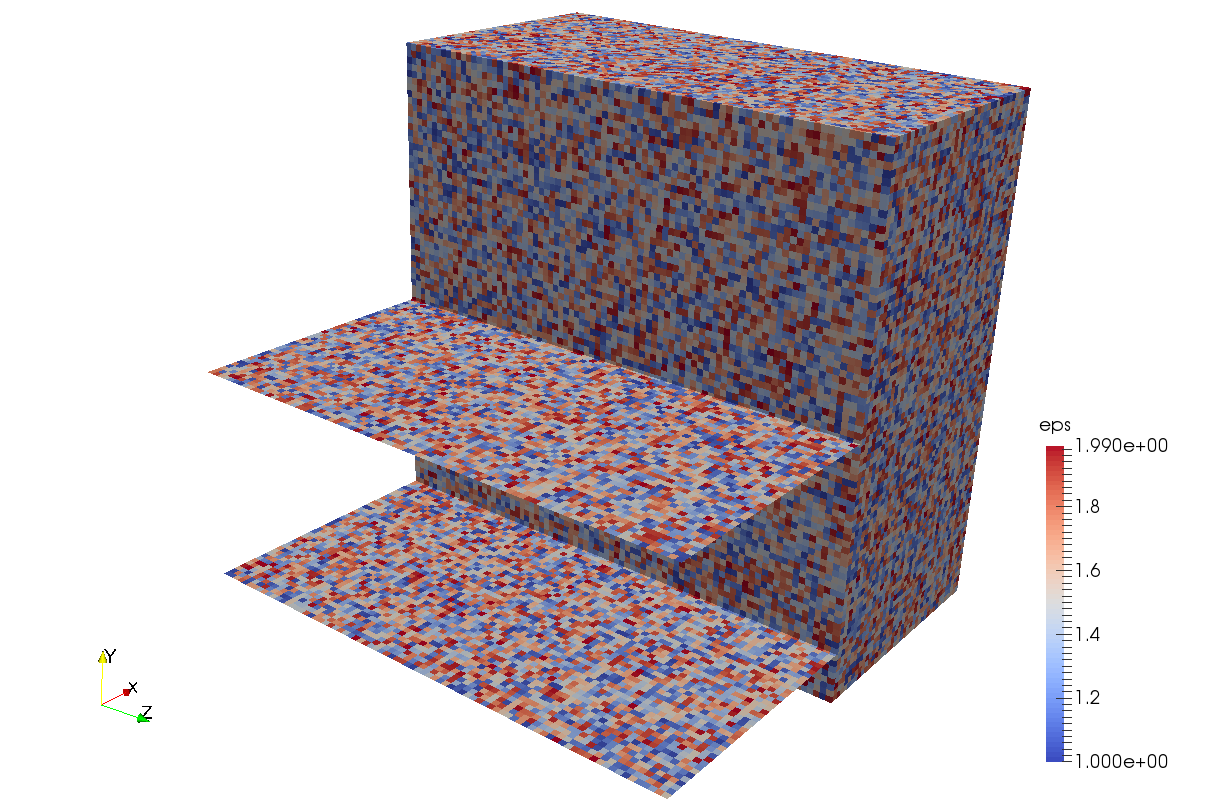
\includegraphics[width=0.7\textwidth]{41_heat-equation/epsilon.png}
\end{center}



\begin{remark}
  It is a `original' decision to model states, vertices and cells as classes
  that actually aggregate their data objects (attribute \texttt{\_stateData},
  \texttt{\_vertexData} or \texttt{\_cellData}, respectively).
  The reason for this is two-fold:
  On the one hand, this allows us to separate user-defined code (the
  aggregating class) from the data model generated by DaStGen. The latter also
  comprises complex technical details such as the MPI data types or bit
  compression. If application-specific code is rewritten, the data model is not
  affected and the other way round. On the other hand, the pattern allows us to
  apply the flyweight pattern. A vertex object is not actually stored and loaded
  from input data. It exists only a few time in total, and in each step its
  change is exchanged underneath by the traversal.
\end{remark}




\subsection{A stencil code}

In this example, we stick to a finite differences formulation and
vertex-centred unknown assignment to do the time stepping.
Our strategy (within the mapping) is simple:
\begin{enumerate}
  \item In \texttt{beginIteration}, we grab the time step size from the state.
  This way, the user might alter the time step size in the outer control loop
  (adaptive time stepping).
  The mapping then always works with the right parameter.
  \item In \texttt{touchVertexFirstTime}, we take the current solution and back
  it up in the vertex's property \texttt{\_oldU}. This property is marked as
  discard, i.e.~the additional helper variable per vertex is not held in-between
  two iterations (actually it is only held for a small number of vertices that
  are still in use). 
  \item In \texttt{enterCell}, we element-wisely accumulate the new solution in
  the vertices.
\end{enumerate}

\begin{code}
class myproject::mappings::TimeStep {
 private:
  /**
   * Logging device for the trace macros.
   */
  static tarch::logging::Log  _log;
    
  double _timeStepSize;
  ...
};


void myproject::mappings::TimeStep::beginIteration(
  myproject::State&  solverState
) {
  logTraceInWith1Argument( "beginIteration(State)", solverState );

  _timeStepSize = solverState.getTimeStepSize();

  logTraceOutWith1Argument( "beginIteration(State)", solverState);
}
\end{code}

\noindent
We reiterate that the state is not available to a mapping by default. If you
need the state (or one of its properties), you explicitly have to grab this data
in \texttt{beginIteration}. As an alternative to the double above, it also would
be possible to copy the whole state. If you want to modify the solver's state,
you have to alter it in \texttt{endIteration}. As Peano requires the user to
explicitly move state data around when required, we ensure that the data remains
consistent in the parallel code variants.

\begin{code}
void myproject::mappings::TimeStep::touchVertexFirstTime(...) {
 ...  
 fineGridVertex.copyCurrentSolutionIntoOldSolution();
 ...  
}

void myproject::Vertex::copyCurrentSolutionIntoOldSolution() {
  _vertexData.setOldU( _vertexData.getU() );
}
\end{code}

\noindent
The interesting stuff happens in the mapping's \texttt{enterCell}, 
where we first of all take all $2^d$ vertices and write their old solution into
one double vector. 
For this, there's a predefined operation in \texttt{VertexOperations} as we have
asked the PDE that we read the scalar.
This $2^d$ vector then is multiplied with the local assembly matrix subject of
an $\epsilon$ scaling.
The result finally is added to the new value.
Again, we us the generated read and write methods.

\begin{code}
#include "myproject/VertexOperations.h"
#include "tarch/la/Matrix.h"

void myproject::mappings::TimeStep::enterCell(...) {
  logTraceInWith4Arguments( "enterCell(...)", fineGridCell, ... );

  tarch::la::Matrix<TWO_POWER_D,TWO_POWER_D,double> A;

  A =  6.0/8.0, -1.0/4.0, -1.0/4.0,      0.0, -1.0/4.0,      0.0,      0.0,      0.0,
      -1.0/4.0,  6.0/8.0,      0.0, -1.0/4.0,      0.0, -1.0/4.0,      0.0,      0.0,
      -1.0/4.0,      0.0,  6.0/8.0, -1.0/4.0,      0.0,      0.0, -1.0/4.0,      0.0,
           0.0, -1.0/4.0, -1.0/4.0,  6.0/8.0,      0.0,      0.0,      0.0, -1.0/4.0,
      -1.0/4.0,      0.0,      0.0,      0.0,  6.0/8.0, -1.0/4.0, -1.0/4.0,      0.0,
           0.0, -1.0/4.0,      0.0,      0.0, -1.0/4.0,  6.0/8.0,      0.0, -1.0/4.0,
           0.0,      0.0, -1.0/4.0,      0.0, -1.0/4.0,      0.0,  6.0/8.0, -1.0/4.0,
           0.0,      0.0,      0.0, -1.0/4.0,      0.0, -1.0/4.0, -1.0/4.0,  6.0/8.0;

  tarch::la::Vector<TWO_POWER_D,double> uOld = 
    VertexOperations::readOldU(fineGridVerticesEnumerator,fineGridVertices);

  const double h = fineGridVerticesEnumerator.getCellSize()(0);

  tarch::la::Vector<TWO_POWER_D,double> uUpdate = 
    - _timeStepSize * fineGridCell.getEpsilon() * A * uOld / h / h  ;

  VertexOperations::writeU(
    fineGridVerticesEnumerator,fineGridVertices,
    VertexOperations::readU(fineGridVerticesEnumerator,fineGridVertices) + uUpdate
  );

  logTraceOutWith1Argument( "enterCell(...)", fineGridCell );
}
\end{code}

\noindent
In this example, I wrote down the local assembly matrix for $d=3$ explicitly.
If you want to support other dimensions, you have to adopt this part
accordingly.

We use Peano's linear algebra routines here.
They are held in the \texttt{tarch} component, and provide all basic
functionality we typically need.
Obviously, it might make sense to switch to other linear algebra packages
(BLAS, e.g.) for more demanding setups.

For a better understanding, it might make sense to have a look into
\texttt{readOldU}.
We note that \texttt{fineGridVertices} is a pointer to an array of vertices, but
the layout of the vertices within this array remains open.
Therefore, Peano hands over an enumerator object. 
The enumerator object has a functor to allow us to select the right vertices.
\texttt{fineGridVertices[ fineGridVerticesEnumerator(0) ]} for example returns
the bottom left vertex of the cell.
See the enumerator's documentation in the header for detailed information.
The read and write that are generated by the PDT run through the vertices and
collect the \texttt{u} or \texttt{oldU} value, respectively, in one vector.
They are scatter/gather operations.
Some codes might prefer not to rely on the temporary vectors and instead work
with the data associated to the vertices directly.
Both options are fine, both options might have different performance
characteristics.

 
Obviously, the above code is not very elaborate. 
The stiffness matrix is set up multiple times.
The most basic optimisation would be to make the matrix an attribute of the
mapping and to initialise it only once.

\begin{remark}
  On the Peano webpage and in the repository, you find a \texttt{matrixfree}
  toolbox. It contains all kind of primitive helper operations that allow you to
  work with stencil codes. It is not as powerful as a real stencil compiler or 
  other matrix-free/PDE toolboxes, but it a small suite to build up at least the
  simpler PDE operators from a finite element/tensor-product formalism and it
  also provides operations fitted to PDT's generated read and write routines. 
The toolbox also provides helper functions that decompose stencils in element-wise
assembly matrices as the one above.
\end{remark}


\noindent
Obviously, our code does not do anything as we do not set any nonzero boundary
conditions. 
Lets do this upon a vertex's first use. 
As we have specified a read, the PDT provides write operations that break up the
object encapsulation.
We make use of this now:

\begin{code}
void myproject::mappings::TimeStep::touchVertexFirstTime(...) {
  ...
  if (fineGridVertex.isBoundary() && fineGridX(0)<1e-8) {
    VertexOperations::writeU( fineGridVertex, 1.0 );
  }
  else if (fineGridVertex.isBoundary()) {
    VertexOperations::writeU( fineGridVertex, 0.0 );
  }
  ...
}
\end{code}

\begin{remark}
In this example, we do not ensure that we do not update boundary vertices.
Indeed, we update them, but in the subsequent traversal we overwrite them again
with the prescribed Dirichlet values (code snippet above). Most codes rather add
an additional if statement checking \texttt{fineGridVertex.isBoundary()}.
\end{remark}

\begin{center}
  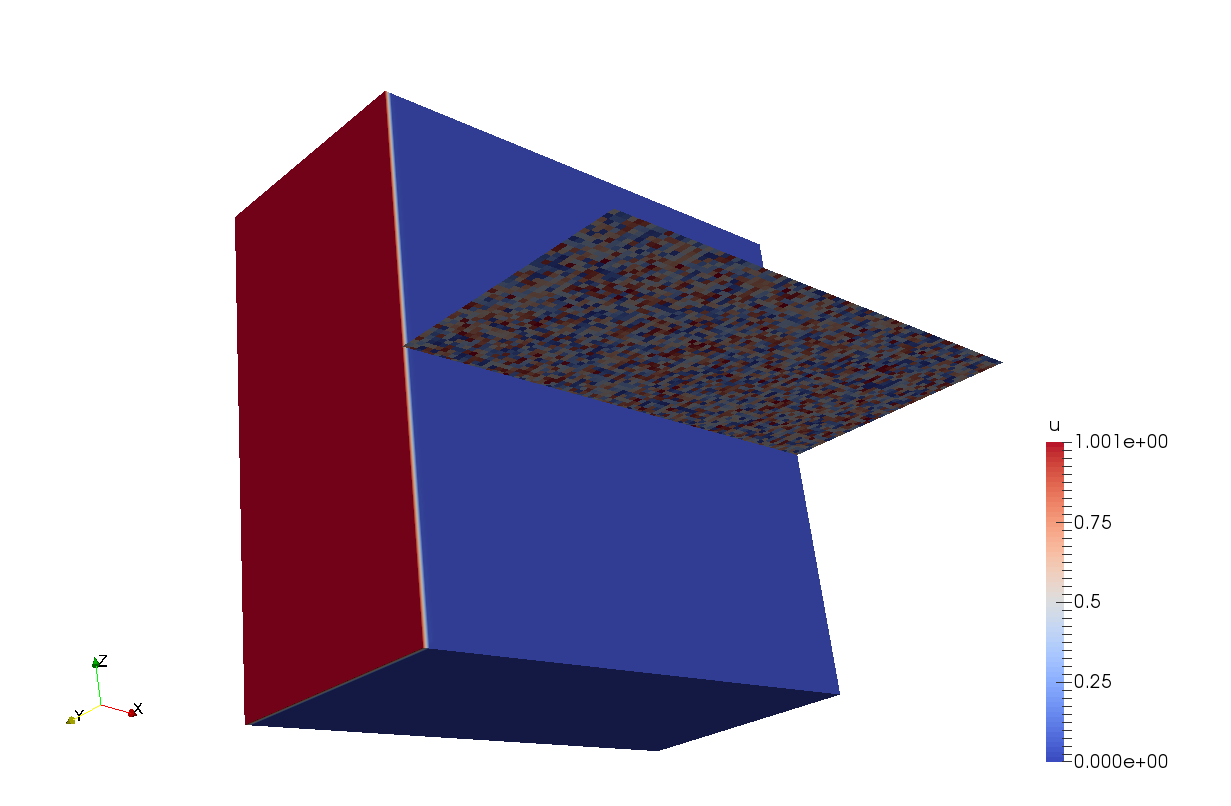
\includegraphics[width=0.45\textwidth]{41_heat-equation/solution00.png}
  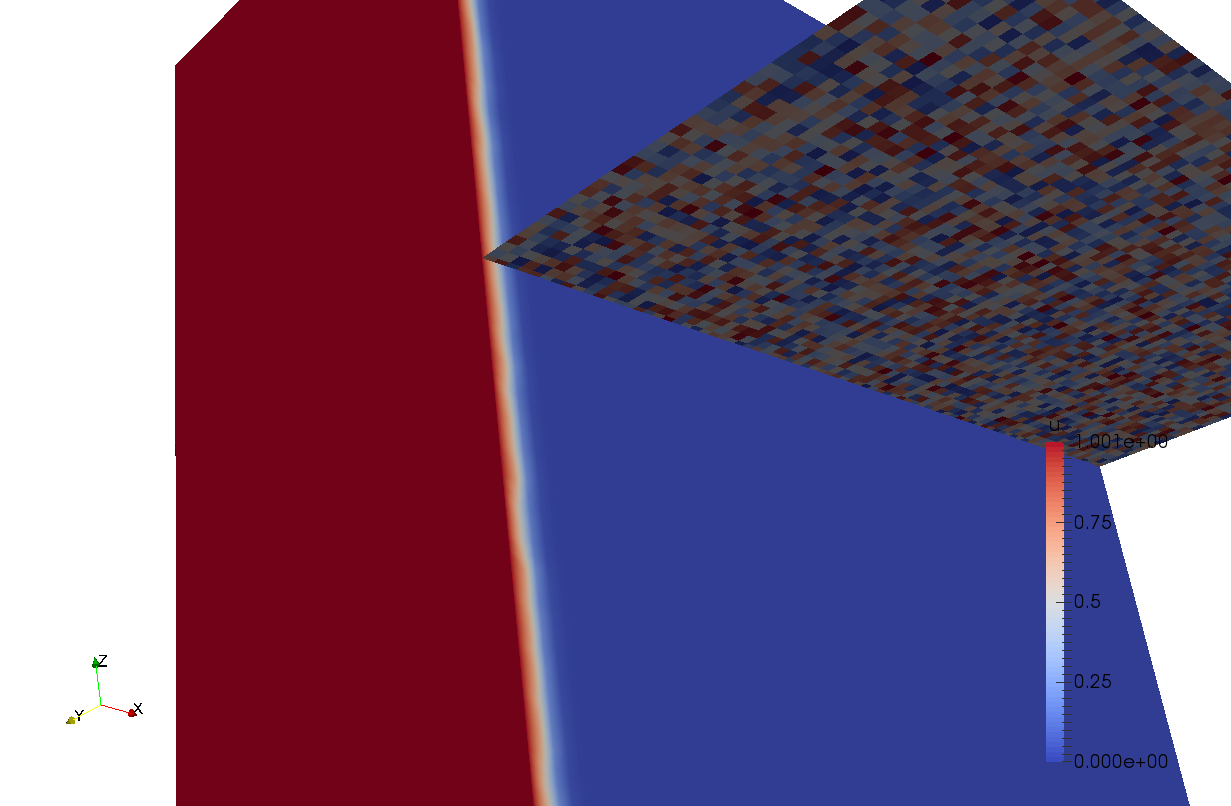
\includegraphics[width=0.45\textwidth]{41_heat-equation/solution01.png}
  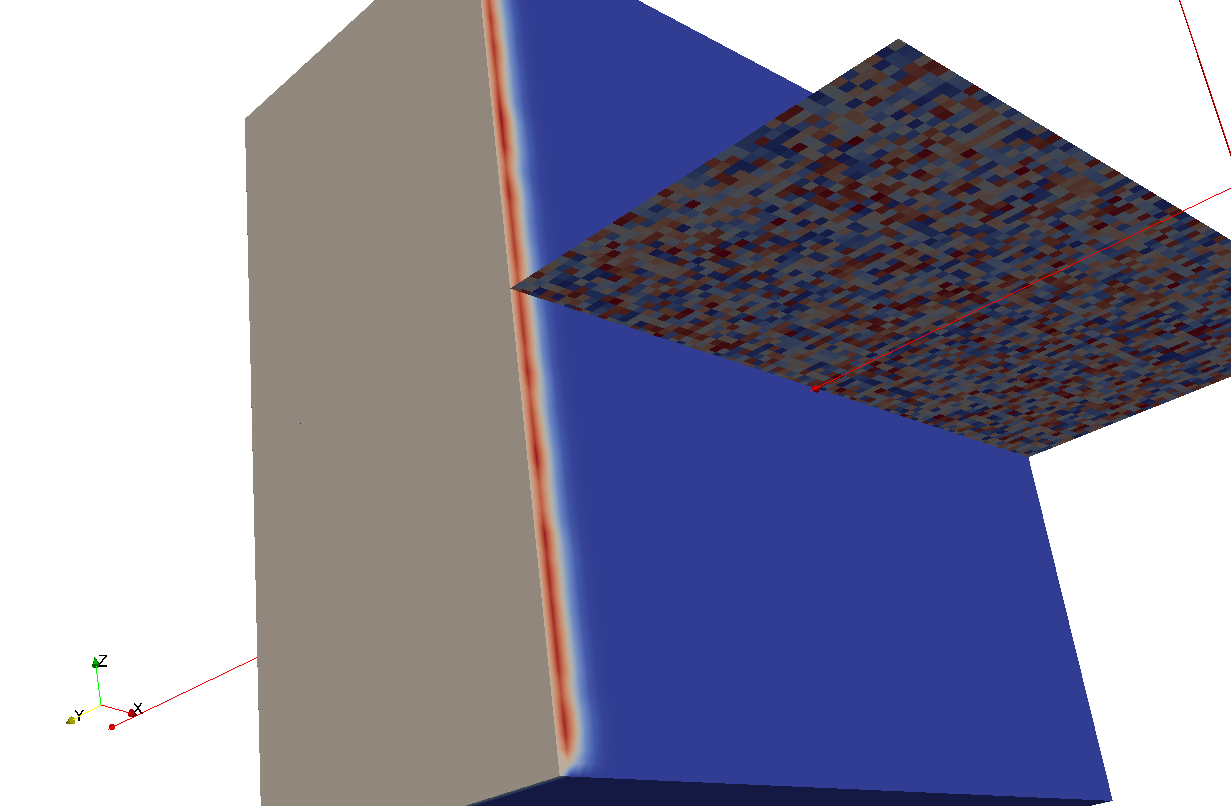
\includegraphics[width=0.45\textwidth]{41_heat-equation/solution02.png}
  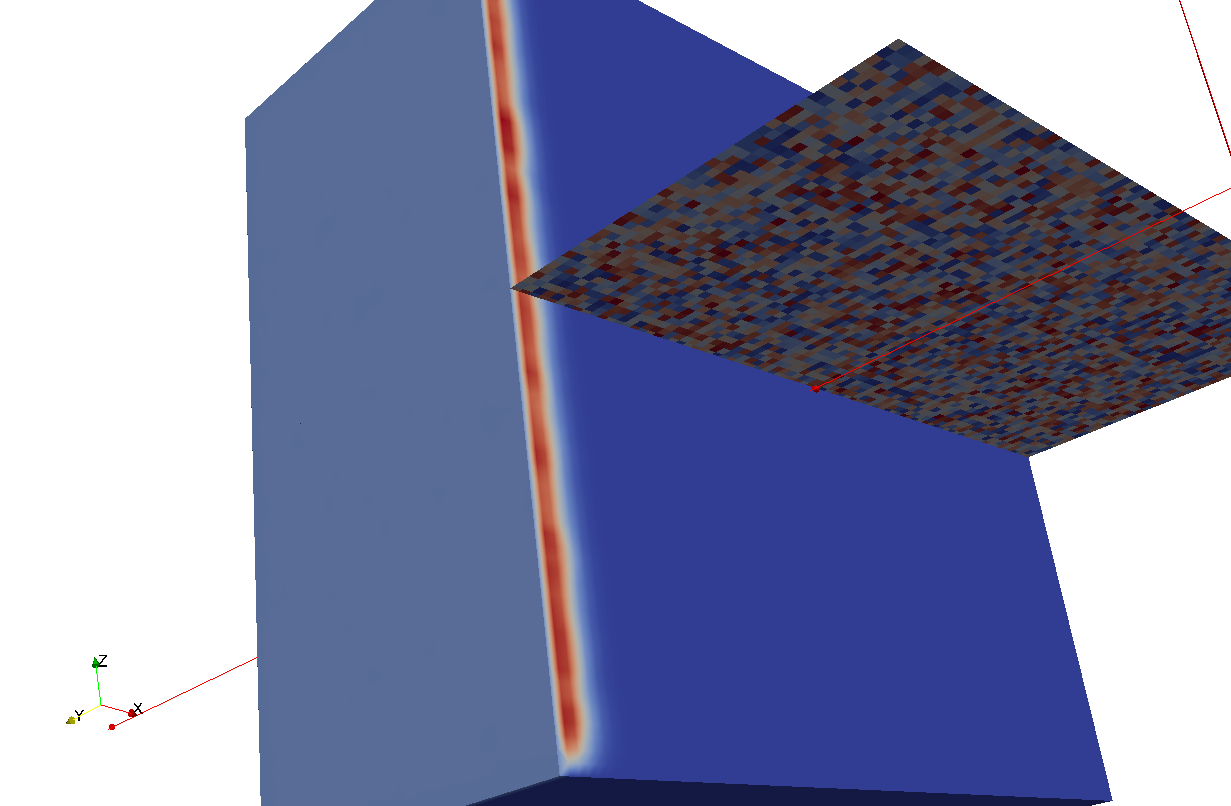
\includegraphics[width=0.45\textwidth]{41_heat-equation/solution03.png}
\end{center}


All figures cut through the domain in the middle and use an orthogonal slice to
visualise the permeability $\epsilon$.
Top, left: We start from a zero condition where only the face at $x=0$ is set to
$1$.
Top, right: Very slowly, the temperature propagates through the domain. As
$\epsilon $ is fuzzy, the propagation profile does not exhibit symmetry but is
ragged as well.
Bottom: The temperature propagates further into the medium.


\subsection{Multiscale data representation}

We continue the solver development with a technical extension that proofs to be
of great value.
Rather than working on the actual fine grid, i.e.~our compute grid, we inject
the finest solutions to the coarser grids all the time:
whenever a vertex coincides with a vertex on a coarser level, we take its value
and copy it to the coarser grid.
To realise this injection, we typically propose to introduce a new mapping in
the specification, and to realise the injection in this new mapping---it has
nothing to do directly with the solver, so the separation of mappings reflects a
separation of concerns.

\begin{code}
...
event-mapping:
  name: Inject
...
adapter:
  name: TimeStep
  merge-with-user-defined-mapping: TimeStep
  merge-with-user-defined-mapping: Inject
...
adapter:
  name: TimeStepAndPlot
  merge-with-user-defined-mapping: TimeStep
  merge-with-user-defined-mapping: Inject
  merge-with-predefined-mapping: VTKPlotVertexValue(result,getU,u)
\end{code}


\noindent
As a result, we have a multiscale representation of the solution on each
individual grid level.
It is (almost) for free, as Peano's vertices are unique due to their combination
of level and spatial position, i.e.~these coarse vertices do exist anyway.

\begin{code}
void myproject::Vertex::inject(const Vertex& fromVertex) {
  _vertexData.setU( fromVertex._vertexData.getU() );
}

void myproject::mappings::Inject::touchVertexLastTime(...) {
 logTraceInWith6Arguments( "touchVertexLastTime(...)", fineGridVertex, fineGridX, ... );

 if ( peano::grid::SingleLevelEnumerator::isVertexPositionAlsoACoarseVertexPosition(
  fineGridPositionOfVertex) ) {
  const peano::grid::SingleLevelEnumerator::LocalVertexIntegerIndex coarseGridPosition = 
   peano::grid::SingleLevelEnumerator::getVertexPositionOnCoarserLevel
   (fineGridPositionOfVertex);

  coarseGridVertices[ coarseGridVerticesEnumerator(coarseGridPosition) ].inject(fineGridVertex);
 }

 logTraceOutWith1Argument( "touchVertexLastTime(...)", fineGridVertex );
}
\end{code}

\noindent
In our implementation, we use helper functions of the enumerator classes. 
Alternatively, we could have checked the integer array
\texttt{fineGridPosiitionOfVertex} manually whether all entries are either 0 or
3.


\begin{remark}
Several projects have exploited this multiscale representation for visualisation
and data postprocessing. Whenever data in a reduced accuracy is sufficient (to
create fancy pictures, e.g.), one can directly extract this data from the
corresponding spacetree level rather than using the finest grid representation
and postprocess these data.
\end{remark}

\subsection{Static adaptivity}

An elegant way to realise adaptive solvers is to pick up the concept of FAC/MLAT
from the multigrid community.
The idea is very simple:
\begin{itemize}
  \item We calculate an update of the solution for each and every cell in the
  sapcetree. This includes the refined ones.
  \item We interpolate hanging nodes from the next coarser levels. This can be
  done recursively, i.e.~a 3:1 balancing of the tree is not required. Rippling
  does not happen.
  \item We inject the solution of a fine grid vertex to the coarser levels and
  thus overwrite the impact of the unknown update there. 
\end{itemize}

\begin{center}
 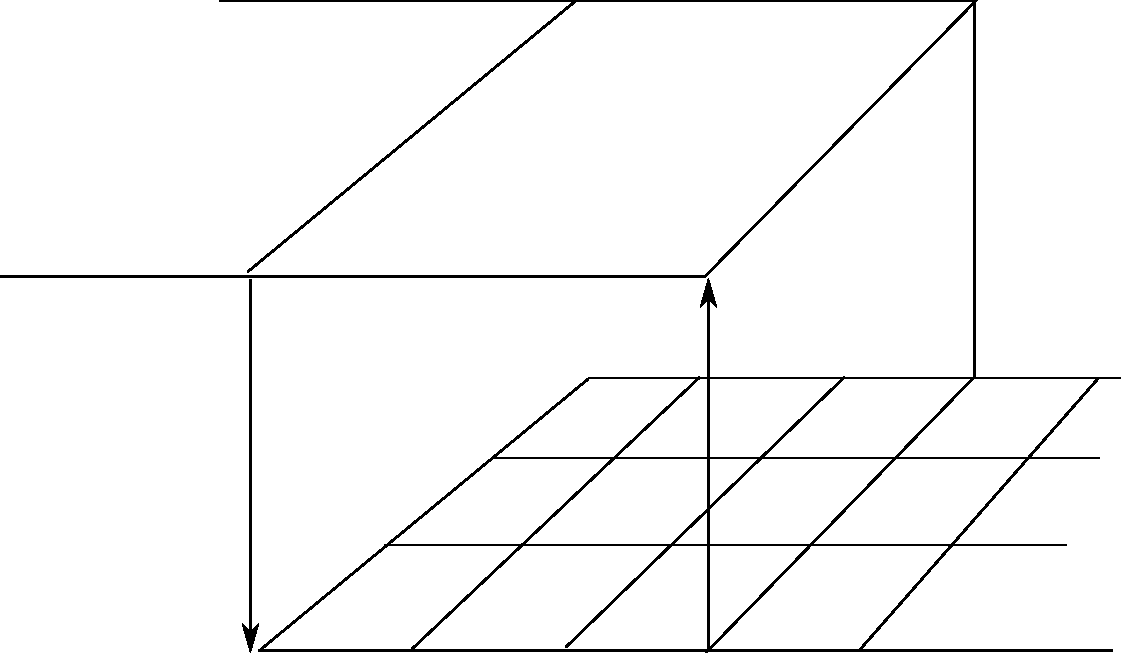
\includegraphics[width=0.34\textwidth]{41_heat-equation/FAC.pdf}
\end{center}


\noindent
One can read such a scheme as an overlapping domain decomposition: 
The coarser levels slightly overlap finer levels. 
Those coarse grid vertices that fall into a fine grid partition are treated as
Dirichlet values (we may update them, but the update then is overwritten
immediately).
Their value is injected from finer grids---an ingredient we already have
realised.
Fine grid problems are handled as Dirichlet problems as well. 
Their boundary points either are real boundary points or hanging nodes.
The value of hanging nodes in turn stems from coarser levels which closes the
coupling of the coarse and fine grid problems.


We propose to introduce---mirroring \texttt{Inject}---a new mapping
\texttt{InterpolateHangingNodes} that solely plugs into the generation of hanging nodes.
This time, we use Peano's $d$-dimensional loops, as well as PDT's generated
write operations that break up the OO encapsulation.

\begin{code}
#include "myproject/VertexOperations.h"
#include "peano/utils/Loop.h"

void myproject::mappings::InterpolateHangingNodes::createHangingVertex(...) {
  logTraceInWith6Arguments( "createHangingVertex(...)", fineGridVertex, fineGridX, ... );

  double interpolatedValue = 0.0;
  dfor2(k)
    double weight = 1.0;
    for (int d=0; d<DIMENSIONS; d++) {
      if (k(d)==0) {
        weight *= 1.0 - (fineGridPositionOfVertex(d))/3.0;
      }
      else {
        weight *= (fineGridPositionOfVertex(d))/3.0;
      }
    }
    interpolatedValue = weight * coarseGridVertices[ coarseGridVerticesEnumerator(k)].getU();
  enddforx

  VertexOperations::writeU( fineGridVertex, interpolatedValue );
  fineGridVertex.copyCurrentSolutionIntoOldSolution();

  logTraceOutWith1Argument( "createHangingVertex(...)", fineGridVertex );
}
\end{code}

\noindent
We reiterate that Peano's \texttt{matrixfree} toolbox provides helpers realising
such typical interpolation tasks.

Finally, we have to setup an adaptive grid. We stick to a static, simple setup
for the time being where the mesh is made very fine along the $x=0$ plane and
reasonably coarse everywhere else.
Please note that you might have to adopt your time step size as well if you
reduce the resolution along the heated up plate.
Furthermore, if you visualise, please note that the default visualiser we used
so far does not know anything about the hanging nodes' interpolation and thus
plots them as zero values. 

\begin{code}
void myproject::mappings::CreateGrid::createInnerVertex(...) {
 if (coarseGridVerticesEnumerator.getLevel()<1) {
  fineGridVertex.refine();
 }
}

void myproject::mappings::CreateGrid::createBoundaryVertex(...) {
 if (coarseGridVerticesEnumerator.getLevel()<3 && fineGridX(0)<1e-8) {
  fineGridVertex.refine();
 }
 else if (coarseGridVerticesEnumerator.getLevel()<1) {
  fineGridVertex.refine();
 }
}
\end{code}


\begin{center}
 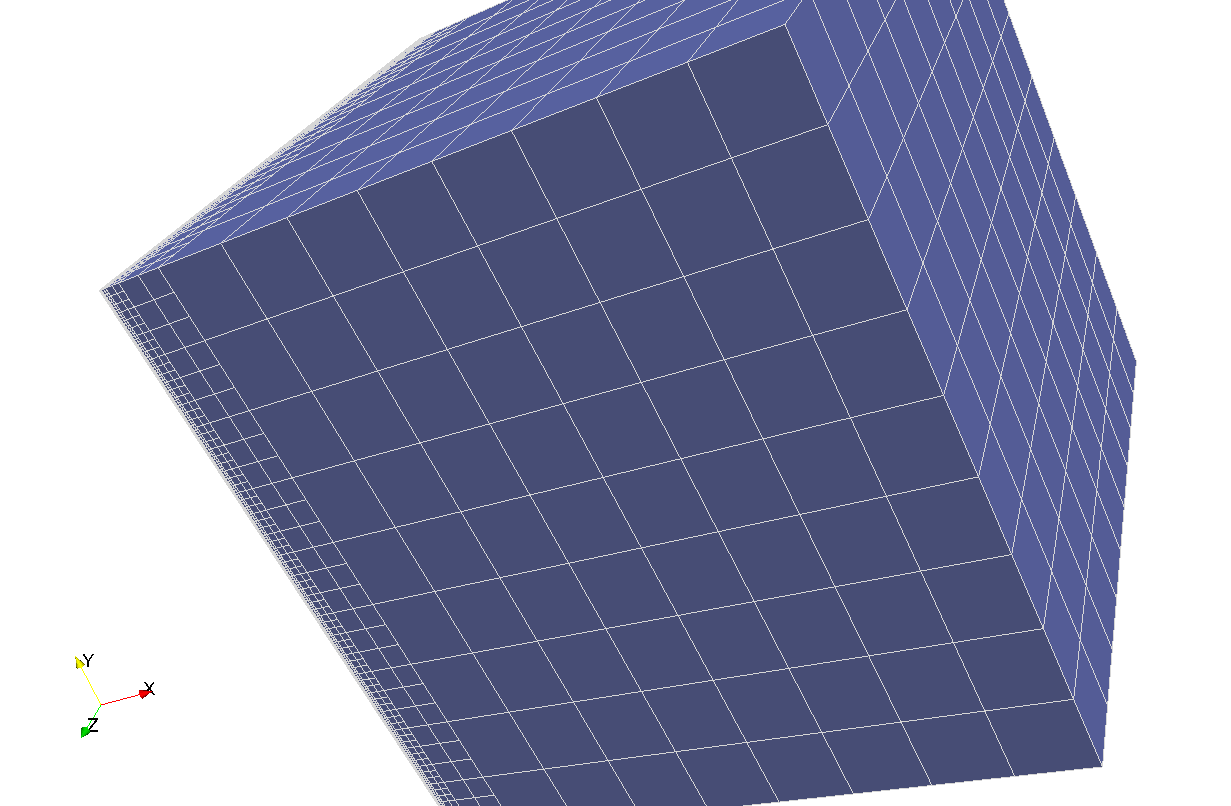
\includegraphics[width=0.45\textwidth]{41_heat-equation/initial-adaptive-grid.png}
 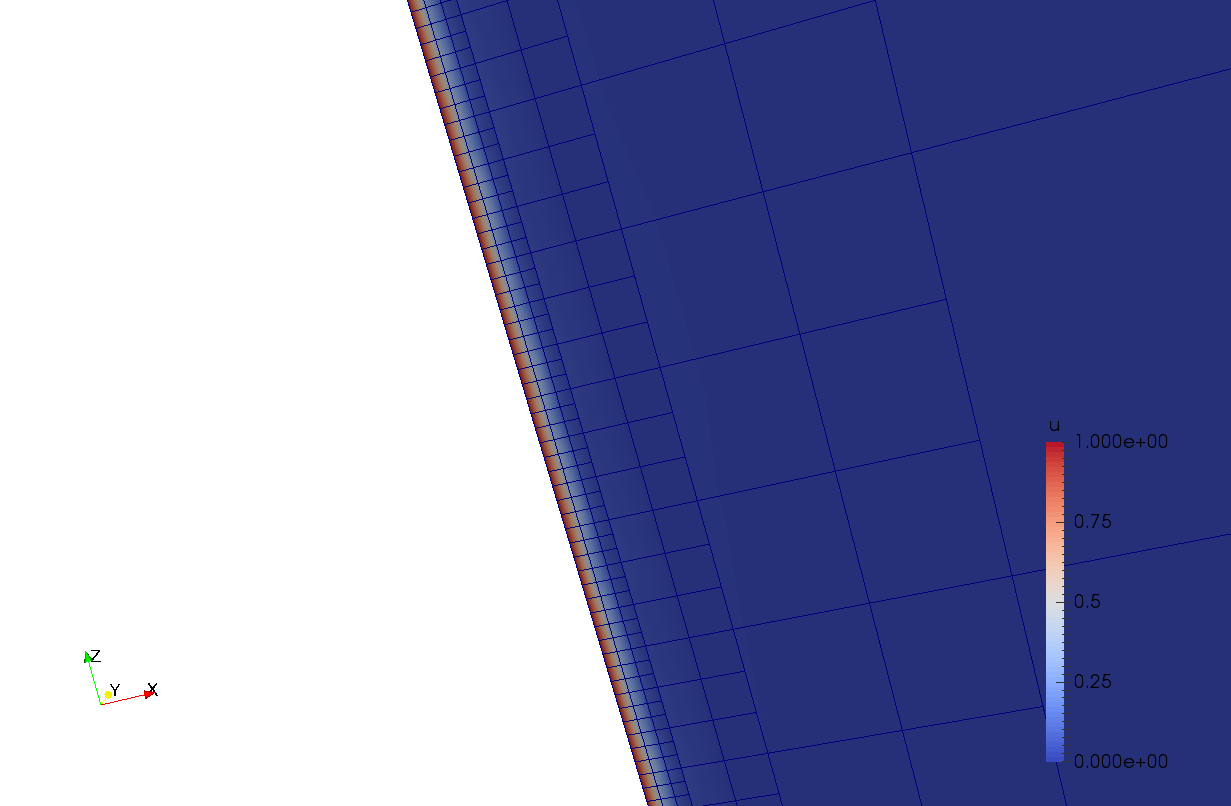
\includegraphics[width=0.45\textwidth]{41_heat-equation/adaptive-grid-21.png}
\end{center}


\noindent
In the present example, it does not matter that some cells compute stencil
evaluations that are never used:
These are the cells where all adjacent vertices are refined.
Due to the injection, the stencil evalution here is not necessary.
As the stencils are very small and cheap to evaluate, this does not make a
difference.
For more complicated setups, it however might make a difference.

Obviously, it is not possible in the present case to use the cells'
\texttt{isRefined()} operation to determine whether a stencil evaluation should
be skipped or not.
Refined cells next to an unrefined one have to be taken into account.
Instead, we have to run over all adjacent vertices of a cell and determine their
refinement state.
Peano realises an or-based refinement---if any vertex adjacent to a cell carries
the refinement bit, the cell is refined---so the required check is an or
combination followed by a negation.
In Peano, there's a class \texttt{peano::grid::aspects::VertexStateAnalysis}.
It is worth to study this class; it offers most of such analysis routines
already and makes the programming of multiscale algorithms more convenient.


\subsection{Dynamic adaptivity}

Given a statically adaptive grid, dynamic adaptivity is (technically) a minor
improvement. 
We realise it in two steps:
\begin{enumerate}
  \item We write the refinement criterion, and 
  \item we ensure that the a posteriori refinement initialises the correct data.
\end{enumerate}

The first step is strongly application dependent. 
A simple criterion that seems to work sufficiently is to assign each vertex a
new (non-persistent) value that holds the average value of the surrounding
vertices. 
If this value differs significantly from the computed value in the point (which
is kind of a smoothness analysis), we refine.
For this, we change the vertex definition
\begin{code}
Packed-Type: short int;


class myproject::dastgen::Vertex {  
  parallelise persistent double  u;
  discard    double  oldU;
  discard    double  averagedU;
};
\end{code}

\noindent
and we also add additional read statements to the specification.
The specification remains more or less unchanged, but we keep all the dynamic
refinement in an additional refinement mapping.

\begin{code}
vertex:
  dastgen-file: Vertex.def
  read scalar(double): U
  read scalar(double): OldU
  read scalar(double): AveragedU
  write scalar(double): U
  write scalar(double): AveragedU
  
...

event-mapping:
  name: RefineDynamically

...

adapter:
  name: TimeStep
  merge-with-user-defined-mapping: TimeStep
  merge-with-user-defined-mapping: Inject
  merge-with-user-defined-mapping: InterpolateHangingNodes
  merge-with-user-defined-mapping: RefineDynamically
\end{code}

\noindent
Before we implement this additional mapping, we create a slightly more appealing
problem setup in create grid:
\begin{code}
void myproject::mappings::CreateGrid::createCell(...) {
  logTraceInWith4Arguments( "createCell(...)", fineGridCell, ... );

  fineGridCell.init( fineGridVerticesEnumerator.getCellCenter() );

  logTraceOutWith1Argument( "createCell(...)", fineGridCell );
}


void myproject::Cell::init(const tarch::la::Vector<DIMENSIONS,double>&  x) {
  _cellData.setEpsilon( x(1) * x(2) + static_cast<double>(rand() % 100)/100.0 );
}
\end{code}

\noindent
Furthermore, we make the start grid one level coarser along the $x=0$ axis 
compared to the previous setup.

Our refinement criterion materialises in a very simple mapping relying on the
simple stencil (here given for two dimensions)
\[
\left[ \begin{array}{ccc}
  0 & 1 & 0 \\
  -1 & 0 & 1 \\
  0 & -1 & 0
\end{array}  \right]
\]
that we apply on the solution.
This stencil determines the derivative in a point.
For a first try, it often yields very reasonable refinement patterns---we
refine where we observe a steep gradient.

\begin{code}
void myproject::mappings::AdaptiveRefinementCriterion::touchVertexFirstTime(...) { 
  logTraceInWith6Arguments( "touchVertexFirstTime(...)", fineGridVertex, ... );

  VertexOperations::writeAveragedU( fineGridVertex, 0.0 );

  logTraceOutWith1Argument( "touchVertexFirstTime(...)", fineGridVertex );
}


void myproject::mappings::AdaptiveRefinementCriterion::enterCell(...) {
  logTraceInWith4Arguments( "enterCell(...)", fineGridCell, ... );

  tarch::la::Matrix<TWO_POWER_D,TWO_POWER_D,double> A;

  A =  0.0,  1.0/4.0,  1.0/4.0,  0.0,  1.0/4.0,  0.0,  0.0,  0.0,
      -1.0/4.0,  0.0,  0.0,  1.0/4.0,  0.0,  1.0/4.0,  0.0,  0.0,
      -1.0/4.0,  0.0,  0.0,  1.0/4.0,  0.0,  0.0,  1.0/4.0,  0.0,
       0.0, -1.0/4.0, -1.0/4.0,  0.0,  0.0,  0.0,  0.0,  1.0/4.0,
      -1.0/4.0,  0.0,  0.0,  0.0,  0.0,  1.0/4.0,  1.0/4.0,  0.0,
       0.0, -1.0/4.0,  0.0,  0.0, -1.0/4.0,  0.0,  0.0,  1.0/4.0,
       0.0,  0.0, -1.0/4.0,  0.0, -1.0/4.0,  0.0,  0.0,  1.0/4.0,
       0.0,  0.0,  0.0, -1.0/4.0,  0.0, -1.0/4.0, -1.0/4.0,  0.0;

  tarch::la::Vector<TWO_POWER_D,double> uOld = 
    VertexOperations::readOldU(fineGridVerticesEnumerator,fineGridVertices);

  const double h       = fineGridVerticesEnumerator.getCellSize()(0);
  const double scaling = 1.0/h;
  tarch::la::Vector<TWO_POWER_D,double> averageUpdate = scaling * A * uOld;

  VertexOperations::writeAveragedU(
    fineGridVerticesEnumerator,fineGridVertices,
    VertexOperations::readAveragedU(fineGridVerticesEnumerator,fineGridVertices) 
    + averageUpdate
  );
 
  logTraceOutWith1Argument( "enterCell(...)", fineGridCell );
}


void myproject::mappings::AdaptiveRefinementCriterion::touchVertexLastTime(...) { 
  logTraceInWith6Arguments( "touchVertexLastTime(...)", fineGridVertex, fineGridX, ... );

  if (coarseGridVerticesEnumerator.getLevel()<6) {
    fineGridVertex.evaluateRefinementCiterion();
  }

  logTraceOutWith1Argument( "touchVertexLastTime(...)", fineGridVertex );
}

\end{code}


\noindent
The magic final operation is kept very simple in this guide book:

\begin{code}
void myproject::Vertex::evaluateRefinementCiterion() {
 if (
  getRefinementControl()==Records::Unrefined
  &&
  std::abs( _vertexData.getAveragedU() )>1.0
 ) {
   refine();
 }
}
\end{code}

\begin{remark}
Almost all sophisticated refinement criteria are based upon a marker concept
such that only a given ratio of the cells are refined per step. 
Such markers are non-trivial to implement as they require global sorting.
It is thus convenient to use some binning approach.
The \texttt{matrixfree} toolbox of Peano has a reference implementation that
also works in an MPI environment.
\end{remark}

For the second step, we have to ensure that all newly created cells and vertices
are intialised correctly.
For the cells, we might simply merge the \texttt{CreateGrid} mapping into our
time stepping adapter.
For the vertices, we have to plug into \texttt{createInnerVertex} where we
initialse the vertex with the interpolated value of its coarse grid parents.
Again, Peano offers toolboxes with routines that do so. 
However, you may also simply reprogram it using the dimension-specific for-loops
of \texttt{Loop.h}.
The routines are then very similar to the interpolation for hanging nodes.
In this example, we do not reuse \texttt{CreateGrid}, but implement everything
within the adaptivity criterion's mapping.

\begin{code}
void myproject::mappings::AdaptiveRefinementCriterion::createCell( ... ) {
  logTraceInWith4Arguments( "createCell(...)", fineGridCell, ... );

  fineGridCell.init( fineGridVerticesEnumerator.getCellCenter() );

  logTraceOutWith1Argument( "createCell(...)", fineGridCell );
}


void myproject::mappings::AdaptiveRefinementCriterion::createInnerVertex( ... ) {
  logTraceInWith6Arguments( "createInnerVertex(...)", fineGridVertex, fineGridX, fineGridH, ... );

  double interpolatedValue = 0.0;
  dfor2(k)
    double weight = 1.0;
    for (int d=0; d<DIMENSIONS; d++) {
      if (k(d)==0) {
        weight *= 1.0 - (fineGridPositionOfVertex(d))/3.0;
      }
      else {
        weight *= (fineGridPositionOfVertex(d))/3.0;
      }
    }
    interpolatedValue = weight * coarseGridVertices[ coarseGridVerticesEnumerator(k)].getU();
  enddforx

  VertexOperations::writeU( fineGridVertex, interpolatedValue );
  fineGridVertex.copyCurrentSolutionIntoOldSolution();

  logTraceOutWith1Argument( "createInnerVertex(...)", fineGridVertex );
}
\end{code}

\noindent
We finally modifiy our runner in two ways:
\begin{enumerate}
  \item We make the runner also plot if the grid changes in a particular time
  step, and
  \item we ensure that the time step size adopts to the grid structure, i.e.~we
  implement adaptive time stepping.
\end{enumerate}

\begin{code}
int myproject::runners::Runner::runAsMaster(myproject::repositories::Repository& repository) {
 peano::utils::UserInterface userInterface;
 userInterface.writeHeader();

 repository.switchToCreateGridAndPlot();
 repository.iterate();
  
 const double initialDt = 1e-4;
 repository.getState().setTimeStepSize( initialDt );
 for (int i=0; i<10000; i++) {
   if (i%100==0 || !repository.getState().isGridStationary()) {
     repository.switchToTimeStepAndPlot();
   }
   else {
    repository.switchToTimeStep();
   }
   repository.iterate();
   double dt = initialDt * repository.getState().getMinimumMeshWidth() 
             * repository.getState().getMinimumMeshWidth();
   repository.getState().setTimeStepSize( dt );
   logInfo( 
    "runAsMaster(...)", 
    "time step " << i << ": dt=" << dt << ", h_min=" <<
    repository.getState().getMinimumMeshWidth() ); 
 }
 
 repository.logIterationStatistics();
 repository.terminate();

 return 0;
}
\end{code}


\noindent
The screenshots below illustrate how the grid evolves in the first four time
steps of the simulation:
\begin{center}
  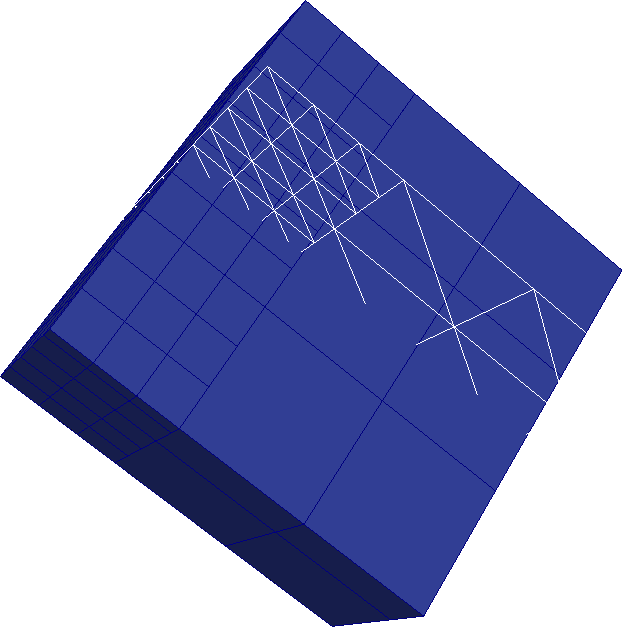
\includegraphics[width=0.4\textwidth]{41_heat-equation/dynamic00.png}
  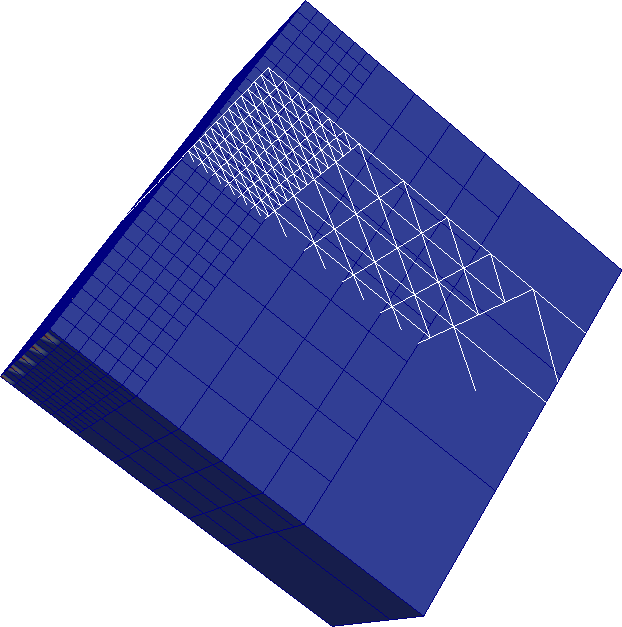
\includegraphics[width=0.4\textwidth]{41_heat-equation/dynamic01.png}
  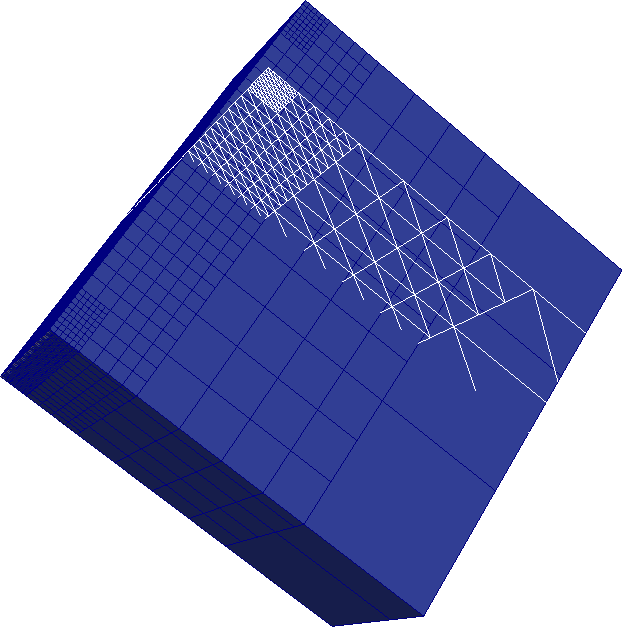
\includegraphics[width=0.4\textwidth]{41_heat-equation/dynamic02.png}
  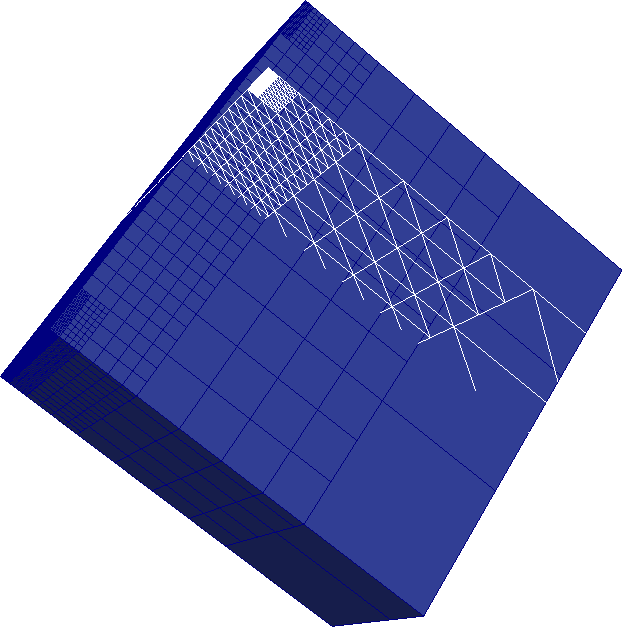
\includegraphics[width=0.4\textwidth]{41_heat-equation/dynamic03.png}
\end{center}


\subsection{Global data}

For most solvers, some kind of global information is required. 
Such data could be 
\begin{itemize}
  \item a global time step size,
  \item a residual norm,
  \item a counter for file plots, 
  \item and so forth.
\end{itemize}

\noindent
We could hold such information as static/global data in our code or as an
attribute in a mapping. 
Both options are not particular appealing. 
Global variables contradict our notion of nice decomposed programming.
Furthermore, I have to anticipate that Peano automatically replicates mappings
on a multithreaded system. 
So we have to be very carefully if we access global data within the mapping's
routines to avoid race conditions.
Attributes of mappings suffer from the same issues.
Furthermore, if mappings are replicated, they are replicated as well: 
instead of data races we have to ensure that data is correctly replicated and
then fused again. 
Finally, if we run on a distributed memory machine, multiple instances of our
application will execute because of MPI's SPMD paradigm, and we have to somehow
manually ensure that global data is kept consistent among all the ranks.


Peano's concept is to model all global data within the \texttt{State.def} file. 
Again, we can here also anticipate which data later on is to be distributed
between different ranks. We have discussed this issue before.
We also have clarified that the standard pattern is to set global data in the
runner through the State object and then to use this data alter on.

\begin{code}
Packed-Type: short int;


class myproject::dastgen::State {  
  persistent parallelise double dt;
};

\end{code}

To use a state, I recommend to make each mapping extract all required data from
the state in \texttt{beginIteration()}.
The idea is as follows (for parallel runs later on): a global algorithm control
routing sets global data in the state.
This state is distributed among all ranks.
All ranks run a particular set of mappings through one adapter.
Each mapping get the required data in \texttt{beginIteration()}.
Later on, we will can tune exactly when the state data is exchanged.

As copying attributes from the \texttt{State} object is laborious, a standard
pattern is to make each mapping hold a copy of the whole state:

\begin{code}
class myproject::mappings::TimeStep {
  private:
    /**
     * Logging device for the trace macros.
     */
    static tarch::logging::Log  _log;

    State _localState;
    ...
};
\end{code}

\noindent
It is important that this state is a local one and is overwritten in each run,
as the runner outside might have changed it.

\begin{code}
void myproject::mappings::TimeStep::beginIteration(
  myproject::State&  solverState
) {
  logTraceInWith1Argument( "beginIteration(State)", solverState );

  _localState  = solverState;
  _localState._clearAttributes(); // see remark below

  assertion2( _timeStepSize>0.0, _timeStepSize, solverState.toString() );

  logTraceOutWith1Argument( "beginIteration(State)", solverState);
}
\end{code}

\noindent
Once you need data from the state, you can extract this data within the mapping
via \linebreak \texttt{solverState.getTimeStepSize()} in the present example.


We finally have to clarify how to collect global data, i.e.~how to realise the
data flow the other way round. 
For this, we also use the copy of the state (this is only one implementation
pattern and again we could fill back data manually attribute-by-attribute. It
is just more convenient this way).
Usually, we first introduce an operation \texttt{State::clearAttributes()} that
resets all data, and we offer operations alike
\texttt{State::updateResidual(double myParam)} that allow us to collect
information within a \texttt{State} instance.

Within the mapping, we then use this operation to collect the data from all grid
entities:
\begin{code}
  ...
  _localState.updateResidual(myValue); 
  ...
\end{code}

\noindent
Obviously, the solution so far is not worth a penny, as the mappings work with
their own local copy of state. 
The solution now is to introduce a new operation 
\begin{code}
void State::merge( const State& otherState ) {
  _stateData.setMyLocalAttribute( 
    _stateData.getMyLocalAttribute() +
    otherState._stateData.getMyLocalAttribute() 
  ); 
}
\end{code}

\noindent
We call this operation in \texttt{endIteration()} to basically backplay the data
from the local copy into the global state:
\begin{code}
void myproject::mappings::TimeStep::endIteration(
  myproject::State&  solverState
) {
  solverState.merge( _localState );
}
\end{code}

\noindent
Finally, we can read the state in the global runner and plot some data to the
terminal, e.g.:
\begin{code}
int myproject::runners::Runner::runAsMaster(myproject::repositories::Repository& repository) {
  ...
  
  const double initialDt = 1e-4;
  repository.getState().setTimeStepSize( initialDt );
  for (int i=0; i<10000; i++) {
    if (i%100==0 || !repository.getState().isGridStationary()) {
      repository.switchToTimeStepAndPlot();
    }
    else {
     repository.switchToTimeStep();
    }
    repository.getState()._clearAttributes();
    repository.iterate();
    logInfo( "runAsMaster(...)", "my fancy global attribute=" <<
    repository.getState().getMyFancyGloalAttribute() );
    
    ...
  }
 
  ...
}
\end{code}

\noindent
Please note that you might have to clear also the global state from time to
time, which is done in the snippet above right before we call \texttt{iterate}.

\begin{remark}
  The whole process seems to be a little bit of overengineering just to get a
  few global variables right. The elegance of the solution becomes obvious when
  we use multiple MPI ranks and multiple threads. There, we rely on exactly the
  same \texttt{merge} operation to distribute a global state first to all ranks
  and threads before we fuse all distributed states together again into one
  object. 
\end{remark}
